We found the feasible activation set for the task of producing nine different sub-maximal magnitudes of static fingertip force in the distal direction, evenly spaced between  $10\%$ and $90\%$ of maximal static force. These are labeled as intensity values $\alpha = 0.1, 0.2., \hdots, 0.9$ in the Figs.  For each sub-maximal force magnitude, we ran 1,000,000 Hit-and-Run iterations and sampled every $100^{th}$ point to produce 10,000 uncorrelated points uniformly distributed in $P$. Recall that for $100\%$ of maximal force $P$ shrinks to a single, unique solution \cite{valero-cuevas2007large}.

\subsection*{Muscle activation histograms}

The histograms in Fig. \ref{fig:raw_histograms} represent the sampled probability distribution of activation for each muscle for the case where the desired fingertip force magnitude in the distal direction is  set to be $\alpha = 0.5$ (i.e., 50% of the maximal possible). 

Fig. \ref{sub:activation_spaces_for_increasing_force} in turn shows  the histograms  all muscles at all nine levels of $\alpha = 0.1$ to $\alpha = 0.9$, as well as the unique solution associated with $\alpha = 1.0$, the  maximal possible  fingertip force in the distal direction. Note that  all histograms include dotted lines indicating the lower- and upper-bounds of sampled activation for each muscle. 

We  validate the Hit-and-Run algorithm by using vertex enumeration methods as in \cite{Valero-Cuevas1998Large,Valero-Cuevas2000Predictive} to find the exact maximal and minimal activation for each muscle (i.e., the individual sides of the bounding box of $P$) at each sub-maximal force level, Figs. \ref{fig:raw_histograms} and \ref{fig:Z_progression}. We found that the difference between the exact and sampled bounds for all muscles was smaller than 0.001, or $<$ 0.1~\% of the $[0, 1]$ range of each muscle. 

\begin{figure}[h]
\centering
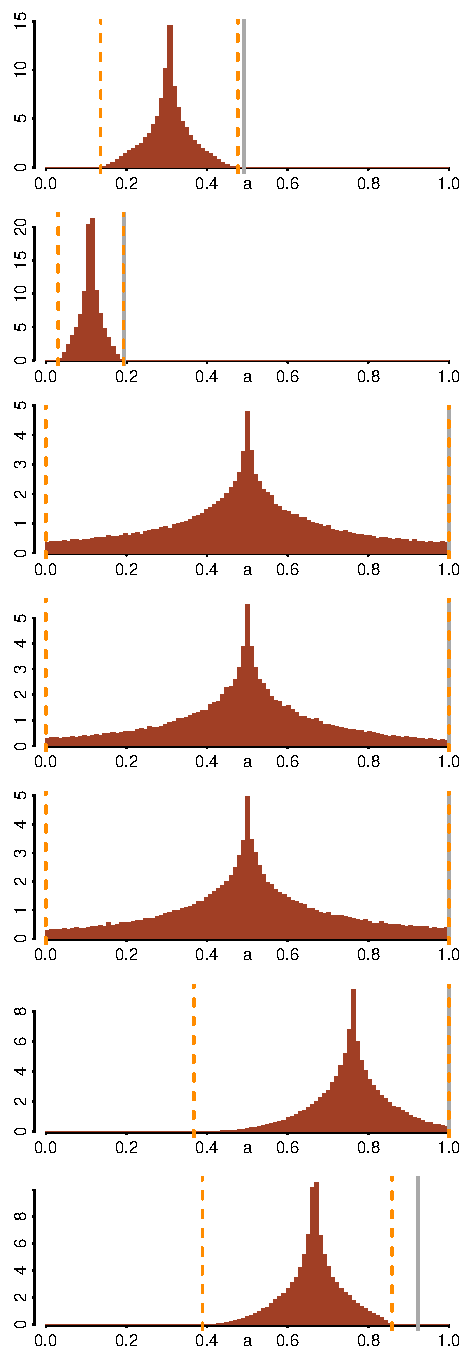
\includegraphics[width=0.5\textwidth]{figs/raw_histograms.pdf}
\caption{Distribution of feasible activations for $\alpha= 0.5$ (50\% of the computed maximal force output in the distal direction). Dashed lines are the observed lower and upper bounds.}
\label{fig:raw_histograms}
\end{figure}



\subsection*{Parallel Coordinates Visualization}
While histograms provide detailed descriptions of the relative density of solutions at various levels of activation for each muscle,  parallel coordinates visualization  effectively shows the relatedness of activation levels across muscles for a given task, magnitude of desired fingertip force, and cost.

We applied parallel coordinate visualization to the 10,000 sampled points for each sub-maximal force level to view how different parts of one muscle's distribution interact with the others.
To maintain real-time interactivity of the plot in our interface, and without perceptible loss of accuracy, we used only the first 1,000 points collected for each task, from $\alpha = 0.1$ to $\alpha = 1.0$. This interactive plot can be seen at \texttt{http://parcoords.divshot.io/examples/slickgrid.html}. Fig. \ref{fig:parcoord_full} shows the parallel coordinate visualization for the same case as in Fig. \ref{fig:raw_histograms}.

\begin{figure}[htbp]
\centering
\includegraphics[width=\textwidth]{figs/parcoord_alpha50.pdf}
\caption{This figure is a snapshot of the interactive platform for visualizing 1000 solutions, all of which produce the same static output force in the distal direction.
This parallel coordinates plot visualizes where each feasible activation set is strewn across each dimension's axis as a line. 
While the activation level $\alpha$ could be set to view all tasks, we set $\alpha$ to a distal force of 50\% of the computed maximal feasible force in this direction. 
Here we show 1,000 points accrued from Hit-and-Run on a task of $\alpha=0.5$.}
\label{fig:parcoord_full}
\end{figure}

Parallel coordinates allow us to visualize not only the proportion of solutions lost when limiting one or more muscle activation or cost function to a given range, but also the location and interrelatedness of the remaining solutions. The density of different solutions is additionally highlighted by the color density resulting from  overlapping  lines. While we invite you to explore the nature of the feasible activation set at the interactive website for yourself, Fig. \ref{fig:parcoords} shows six such explorations.

\begin{figure}[htbp]
\centering
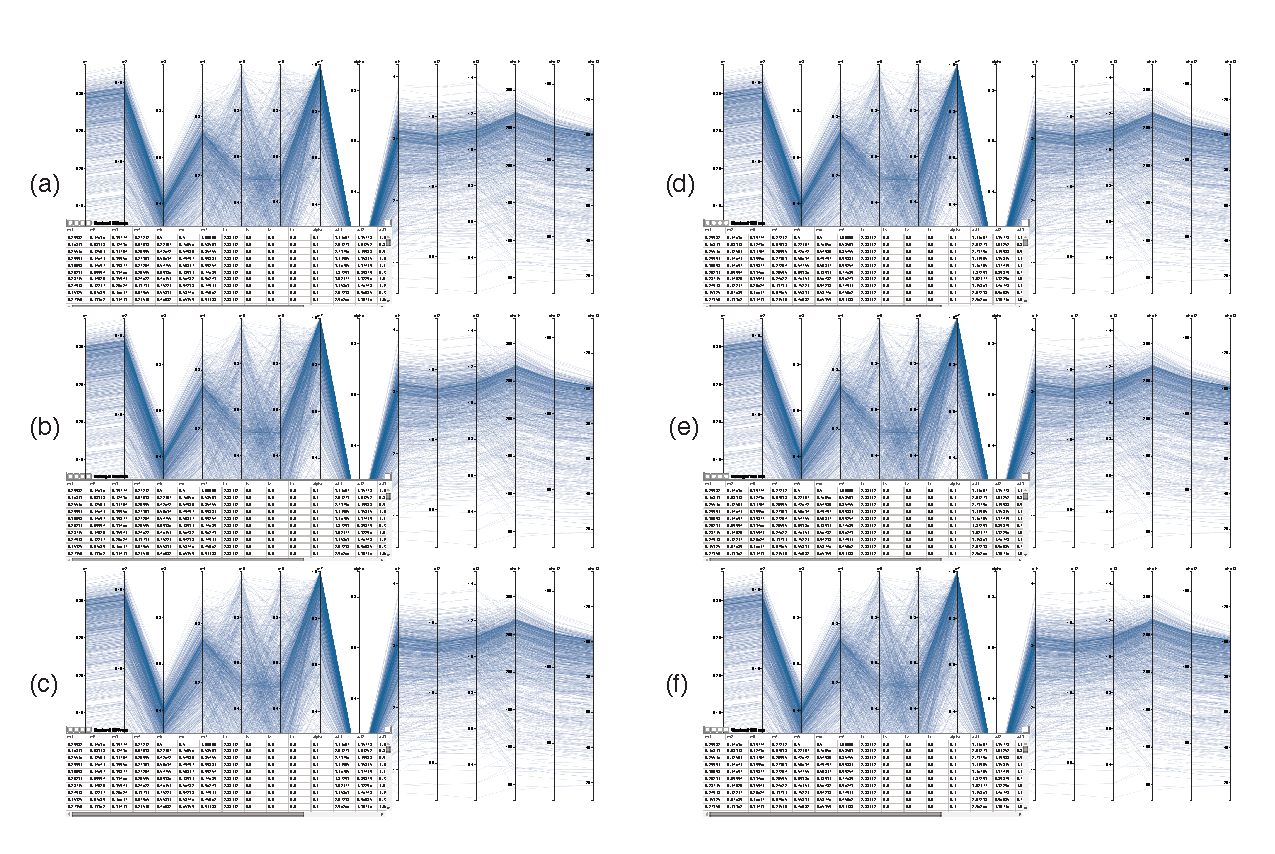
\includegraphics[width=\textwidth]{figs/parcoords.pdf}
\caption{These snapshots show the use of the interactive parallel coordinate visualization of solutions across the activation space. For the task set to 50\% of maximal in the distal direction, we show the
(a) remaining 166 solutions when PI $<$ 60\% 
(b) remaining 57 solutions when DI $<$ 60\%, and the
(c) remaining 57 solutions when we constrain PI $<$ 60\% and DI $<$ 60\%. We also show the
(d) remaining 502 solutions when we select the lower 50\% of $L_1$ costs,
(e) remaining 498 solutions when we select the lower 50\% of $L_2^w$ costs, and the
(f) remaining 220 solutions when we select the lower 50\% across all cost functions in Table \ref{cost_function_tabls} }
\label{fig:parcoords}
\end{figure}

Constraining PI $<$ 60\% still leaves a solution space about three times as large as di $<$ 60\%. 
Observe that constraining DI $<$ 60\% already implies that PI $<$ 60\% as seen in Fig. \ref{fig:parcoords} (b), (c). 
Constraining one muscles does have different effects on the other muscles as for example if ei is constrained below 60\% activation, we see that the bounding box of PI is significantly restricted; however, the same constraint has no effect on the bounding box of EIP.

As there are few steep crossings between $L_1$, $L_2$ and $L_3$, the parallel coordinates suggest correlation of those three cost functions.
Similar correlation is observed for the respective weighted functions.
We provide a scatter plot for their relationships in Appendix Fig. \ref{fig:unweighted_cost_functions} and \ref{fig:weighted_cost_functions}.

% subsection paralleL_coordinates (end)



\subsection*{Changes in the structure of the feasible activation space with increasing force mangitude, a.k.a. how muscle redundancy is lost} % (fold)
\label{sub:activation_spaces_for_increasing_force}
The maximal static fingertip force into any direction (i.e., at $\alpha=1$) is produced by  a unique combination of muscle activations \cite{spoor1983balancing,Chao1978Graphical,valero-cuevas2015fundamentals}. Therefore, the histograms in Fig. \ref{fig:Z_progression} show how the multiple solutions available for sub-maximal forces change and shrink  for increasing force magnitude, from $\alpha=0.1$  to $\alpha=1$. You can track the change in the feasible distributions of a given muscle's activations by following its column from top to bottom ending, naturally, with the unique value needed for maximal force magnitude. 

\begin{figure}[htbp]
\centering
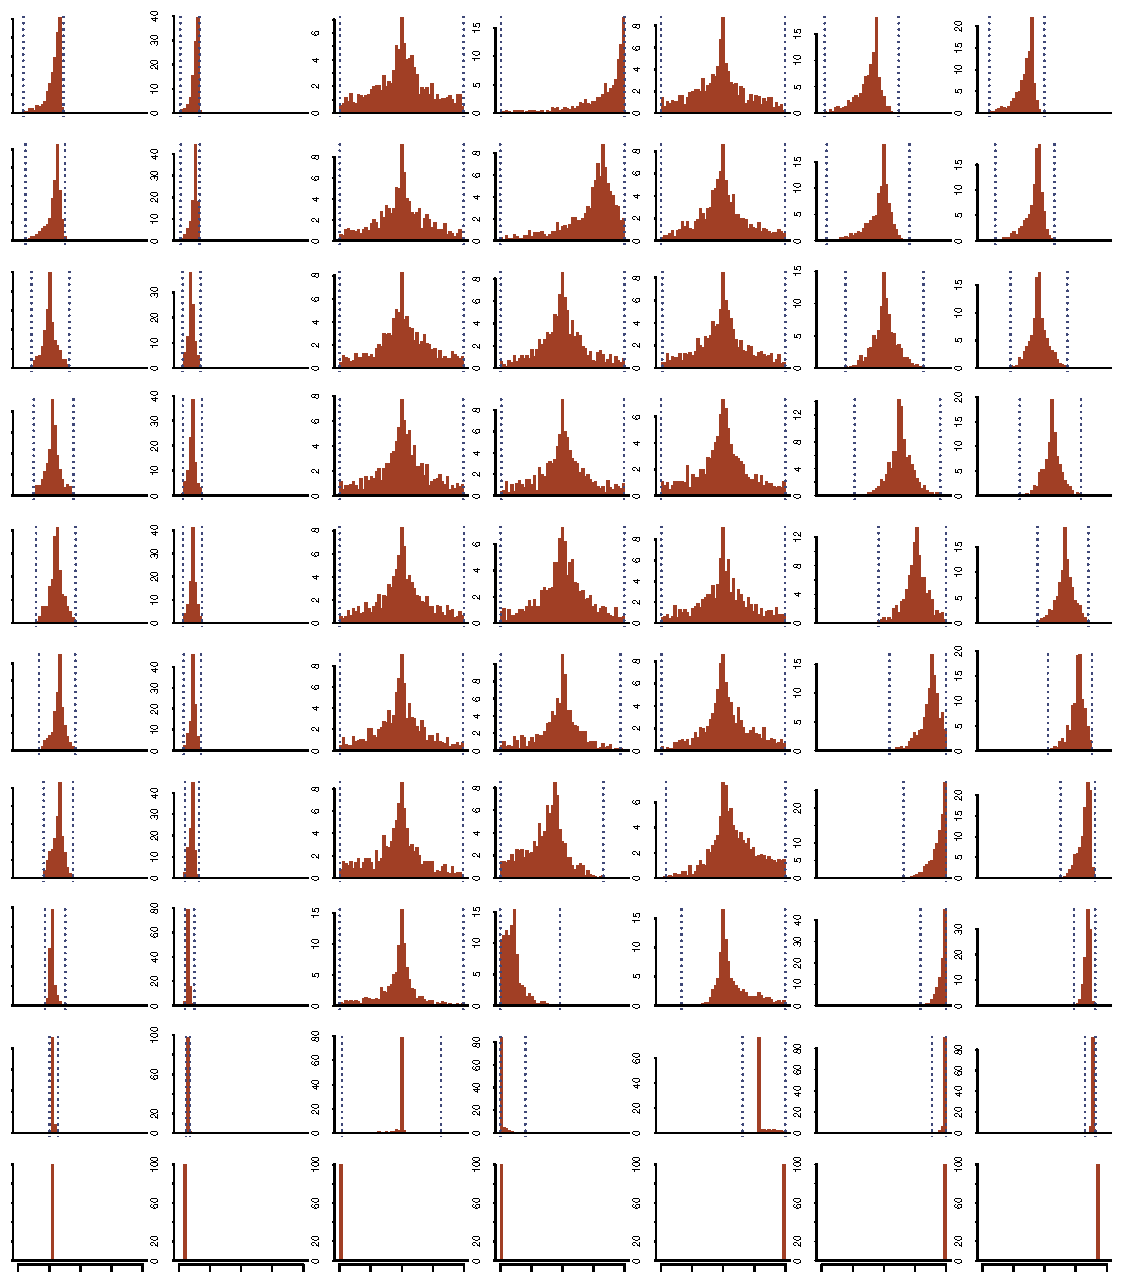
\includegraphics[width=\textwidth]{figs/Z_alphaProgression1430924065026.pdf}
\caption{Distribution of activations in the distal direction and changing force. Each row of histograms uses a Hit-and-Run set. The height of each bar visualizes the percentage of 10,000 solutions found within a given bins that are 0.02 wide (i.e., 2\% of total activation range $[0,1]$).  The shape is as meaningful than the height of individual bins of the histograms. Of note is that the mode of the sub-maximal histograms changes, and is seldom the equivalent of the unique activation value needed to achieve maximal force. The lower- and upper-bounds of the histograms are shown as  vertical dotted lines. [what is that other vertical lines]. To our knowledge this is the first time that the internal structure of the feasible activation set has been visualized.}
\label{fig:Z_progression}
\end{figure}

The solution polytope converges as the difficulty of the task increases; the rate of convergence is different across muscles.
For some muscles the convergence only occurs after $\alpha=0.6$ or $\alpha=0.8$ (as in LUM and EIP), while others converge across the entire progression (e.g.\ DI and PI).
Whereas for example FDS already has a small range of feasible activations at $\alpha=0.1$, EIP has feasible activation $[0,1]$ up to 80\%.

It is imperative to keep in mind that every histogram (regardless of its convergence) is composed of the distribution of all 10,000 points; when the distribution is compressed, the relative percentage of the bars will increase (as evident by the increasing y-axis limits), as we fixed break width ($\Delta x$) to remain constant to 2\% of maximal activation \cite{ball1997elementary}.

The peaks seen in these figures is the perpendicular slice that has the largest relative volume; within the same muscle it does not have to be symmetric between the bounds, and can shift over differing tasks.
As expected, the unique solution at $\alpha=1.0$ appears as a single peak representing 100\% of the sampled points; the bounds and the muscle's unique activation are superimposed.

The most simple finding is that the distributions cannot be inferred by their bounding boxes alone.
Consider the activation distributions between $\alpha = 0.7$ and $\alpha = 0.8$ for LUM, where the median changed by less than 4\% while the lower bound increased by nearly 13\%.
Notably, we observe that a meaningful cross-muscle comparison of point distributions cannot be ascertained by the bounding box. For example, at a task of 10\% of maximal distal force production, EIP and EDC both have lower and upper bounds of 0, and 1, respectively, yet their distributions are thoroughly distinct; the shape of EIP is more symmetric (lower 25\% = 0.36, median = 0.5029, upper 75\% = 0.62), while 75\% of the solutions sampled have EDC higher than 0.74 (see Fig. \ref{fig:Z_progression}).

We find this holds not only for inter-muscle distribution comparisons, but intra-muscular distributions. Consider the significant change in the shape of the distributions across the progression for EDC until the 60\% task; the lower and upper bounds change less than 1\% and 4\%, respectively, while the median shifted by nearly 40\%.
In the most extreme case, the median activation can be exceptionally narrow, while the bounds are wide- for example, EIP at a 90\% task; although activation is bounded between 0.1 and 0.81, approximately 79\% of the solutions exist with EIP activation between just 0.49 and 0.51.

Next, we see that if one muscle had to be fixed throughout the entire force progression, DI and PI would fail; their bounding boxes of tasks below $\alpha=0.4$ do not include the unique solution at $\alpha=1.0$.
We also placed a vertical grey line for the scaled unique solution at maximal force, denoted $\textbf{a}^*$, (e.g. LUM converges to an activation of 1 at maximal distal force, so we put a grey line at 0.8 for $\alpha=0.8$ of maximal distal force).
Since $\alpha \textbf{f}_{\max} = \alpha A \textbf{a}^*$, $\alpha \textbf{a}^*$ is a solution of the feasible activation set at $\alpha$-fraction of the maximal force.
However we observe that for some muscles, these points can lie arbitrarily in the distribution i.e.\ do not have to lie close to the corresponding peaks (e.g.\ musle DI and EIP).



